    This section provides a detailed plan for the implementation, integration, and testing of the S\&C platform. The first section will describe the main concepts and ideas behind the Implementation, Integration and Test plan and the following sections will provide a description for each step of it. 
    \subsection{Plan Overview}
    The platform will be implemented, integrated and tested following a mix between a \textit{thread} and \textit{bottom-up} approach thanks to the aforementioned microservices architecture that allows different service to be implemented and tested in parallel with others.\\
    The main idea is to develop one feature of the Platform Logic at a time, whenever possible, by implementing the front-end user interface (UI) and the back-end corresponding components and the notifications they will generate. Each feature will undergo unit testing before being integrated with other components. By adopting this thread-based implementation, we can begin testing component integration early in the development process, instead of waiting for the entire Platform Logic to be completed. We believe that this approach allows us to identify and resolve integration issues at an earlier stage, minimizing the risk of significant problems arising later on.\\
    However, due to dependency constraints, not all components can be developed using this thread-based approach. For example, the Recommendation Process and Suggestion Mechanism relay to the User Manager and Platform Entity Manager. To address this, the “Implementation, Integration and Test Plan” is organized into several steps, following a bottom-up approach dividing components into groups that can be developed, tested, and integrated independently.
    \subsection{Plan Stage}
    \subsubsection{Stage 1: User Manager and Notification Manager}
    In the first stage, we will develop the User Manager and part of the Notification Manager, enabling each component to store and retrieve data from its respective database. This process will also involve developing the Platform Entity Manager and the Notification Entity Manager so that each can interact with its own database. To test these two components, we will create an API controller DRIVER and a Manager DRIVER to simulate API controller calls and the various invocations from other components within the Platform Logic.\\ 
    \begin{figure}[H]
    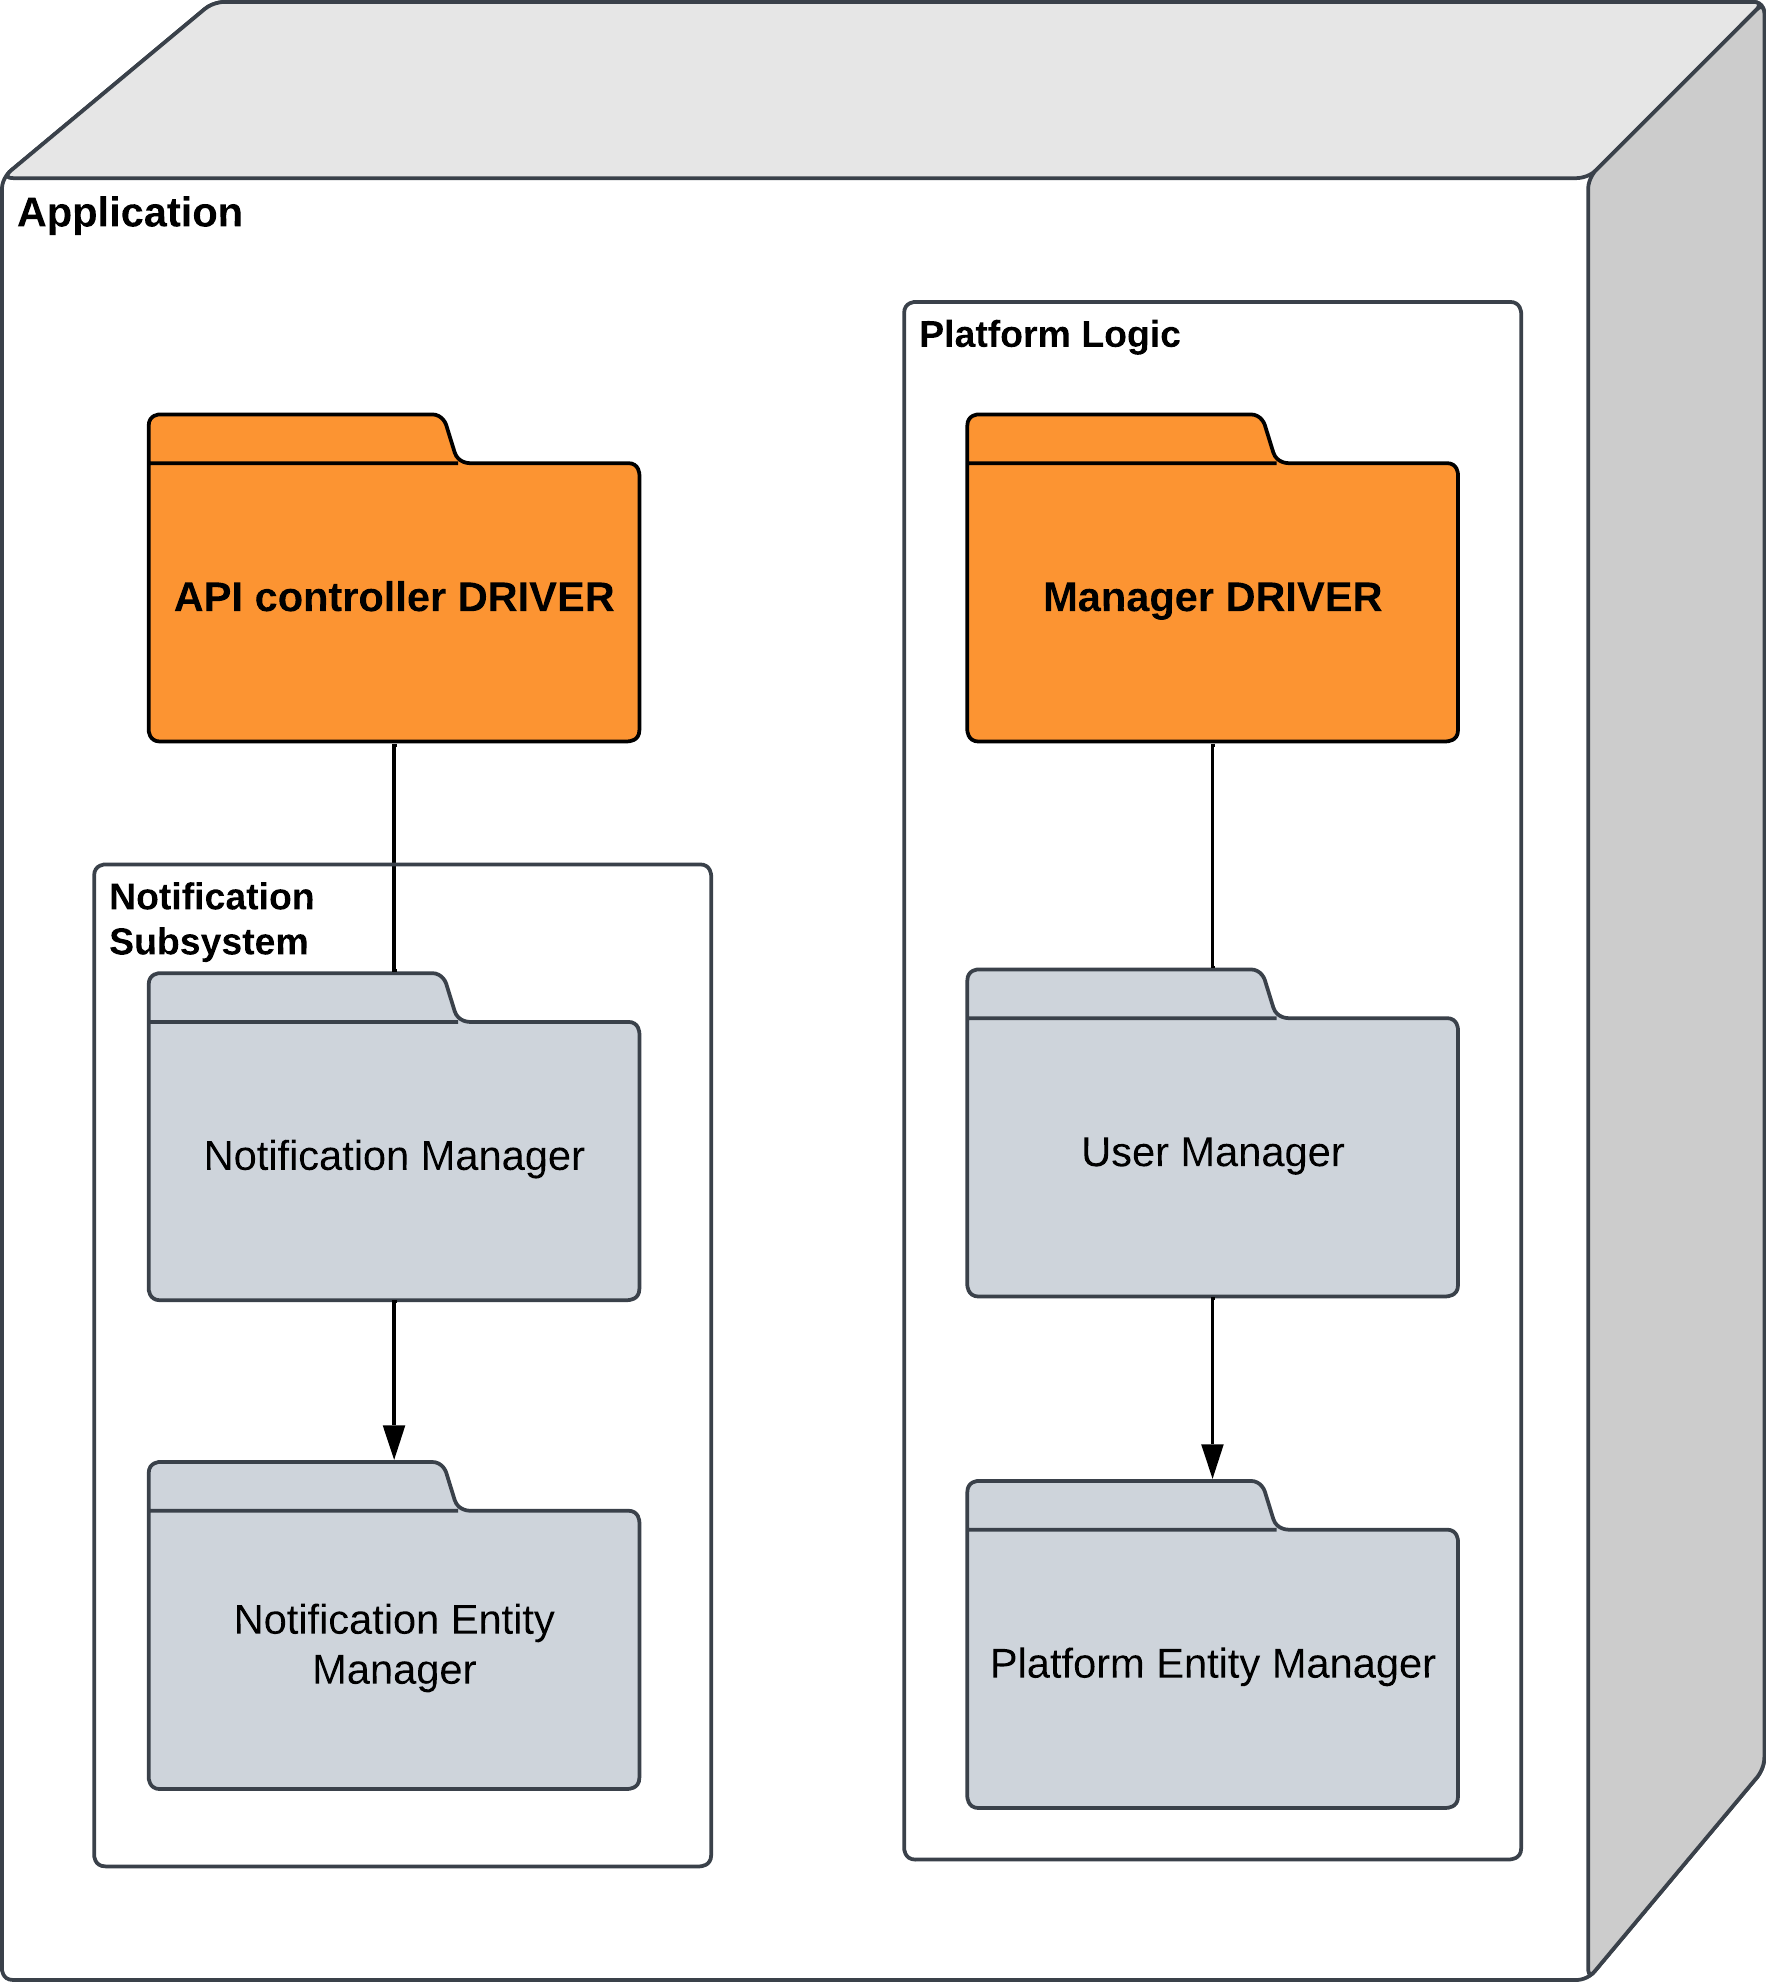
\includegraphics[width=0.35\linewidth]{Latex/Images/DD/Testing/TestingPlanStep1.png}
    \centering
    \caption{User Manager and Notification Manager testing}
    \label{fig:test-step1}
    \end{figure}
    
    \subsubsection{Stage 2: Platform Logic Components and User Interface}
    In the second stage, we will develop the remaining Platform Logic components, including the Recommendation Process, Mechanism components, and the remaining Managers. During this phase, we will also implement the User Interface (UI) and update the Notification Manager to handle notifications sent by these components, following the idea behind the \textit{thread} approach. To test these back-end components, we will create an API Controller DRIVER to simulate their invocation, while creating a Rest API STUB to simulate the front-end calls.\\
    \begin{figure}[H]
    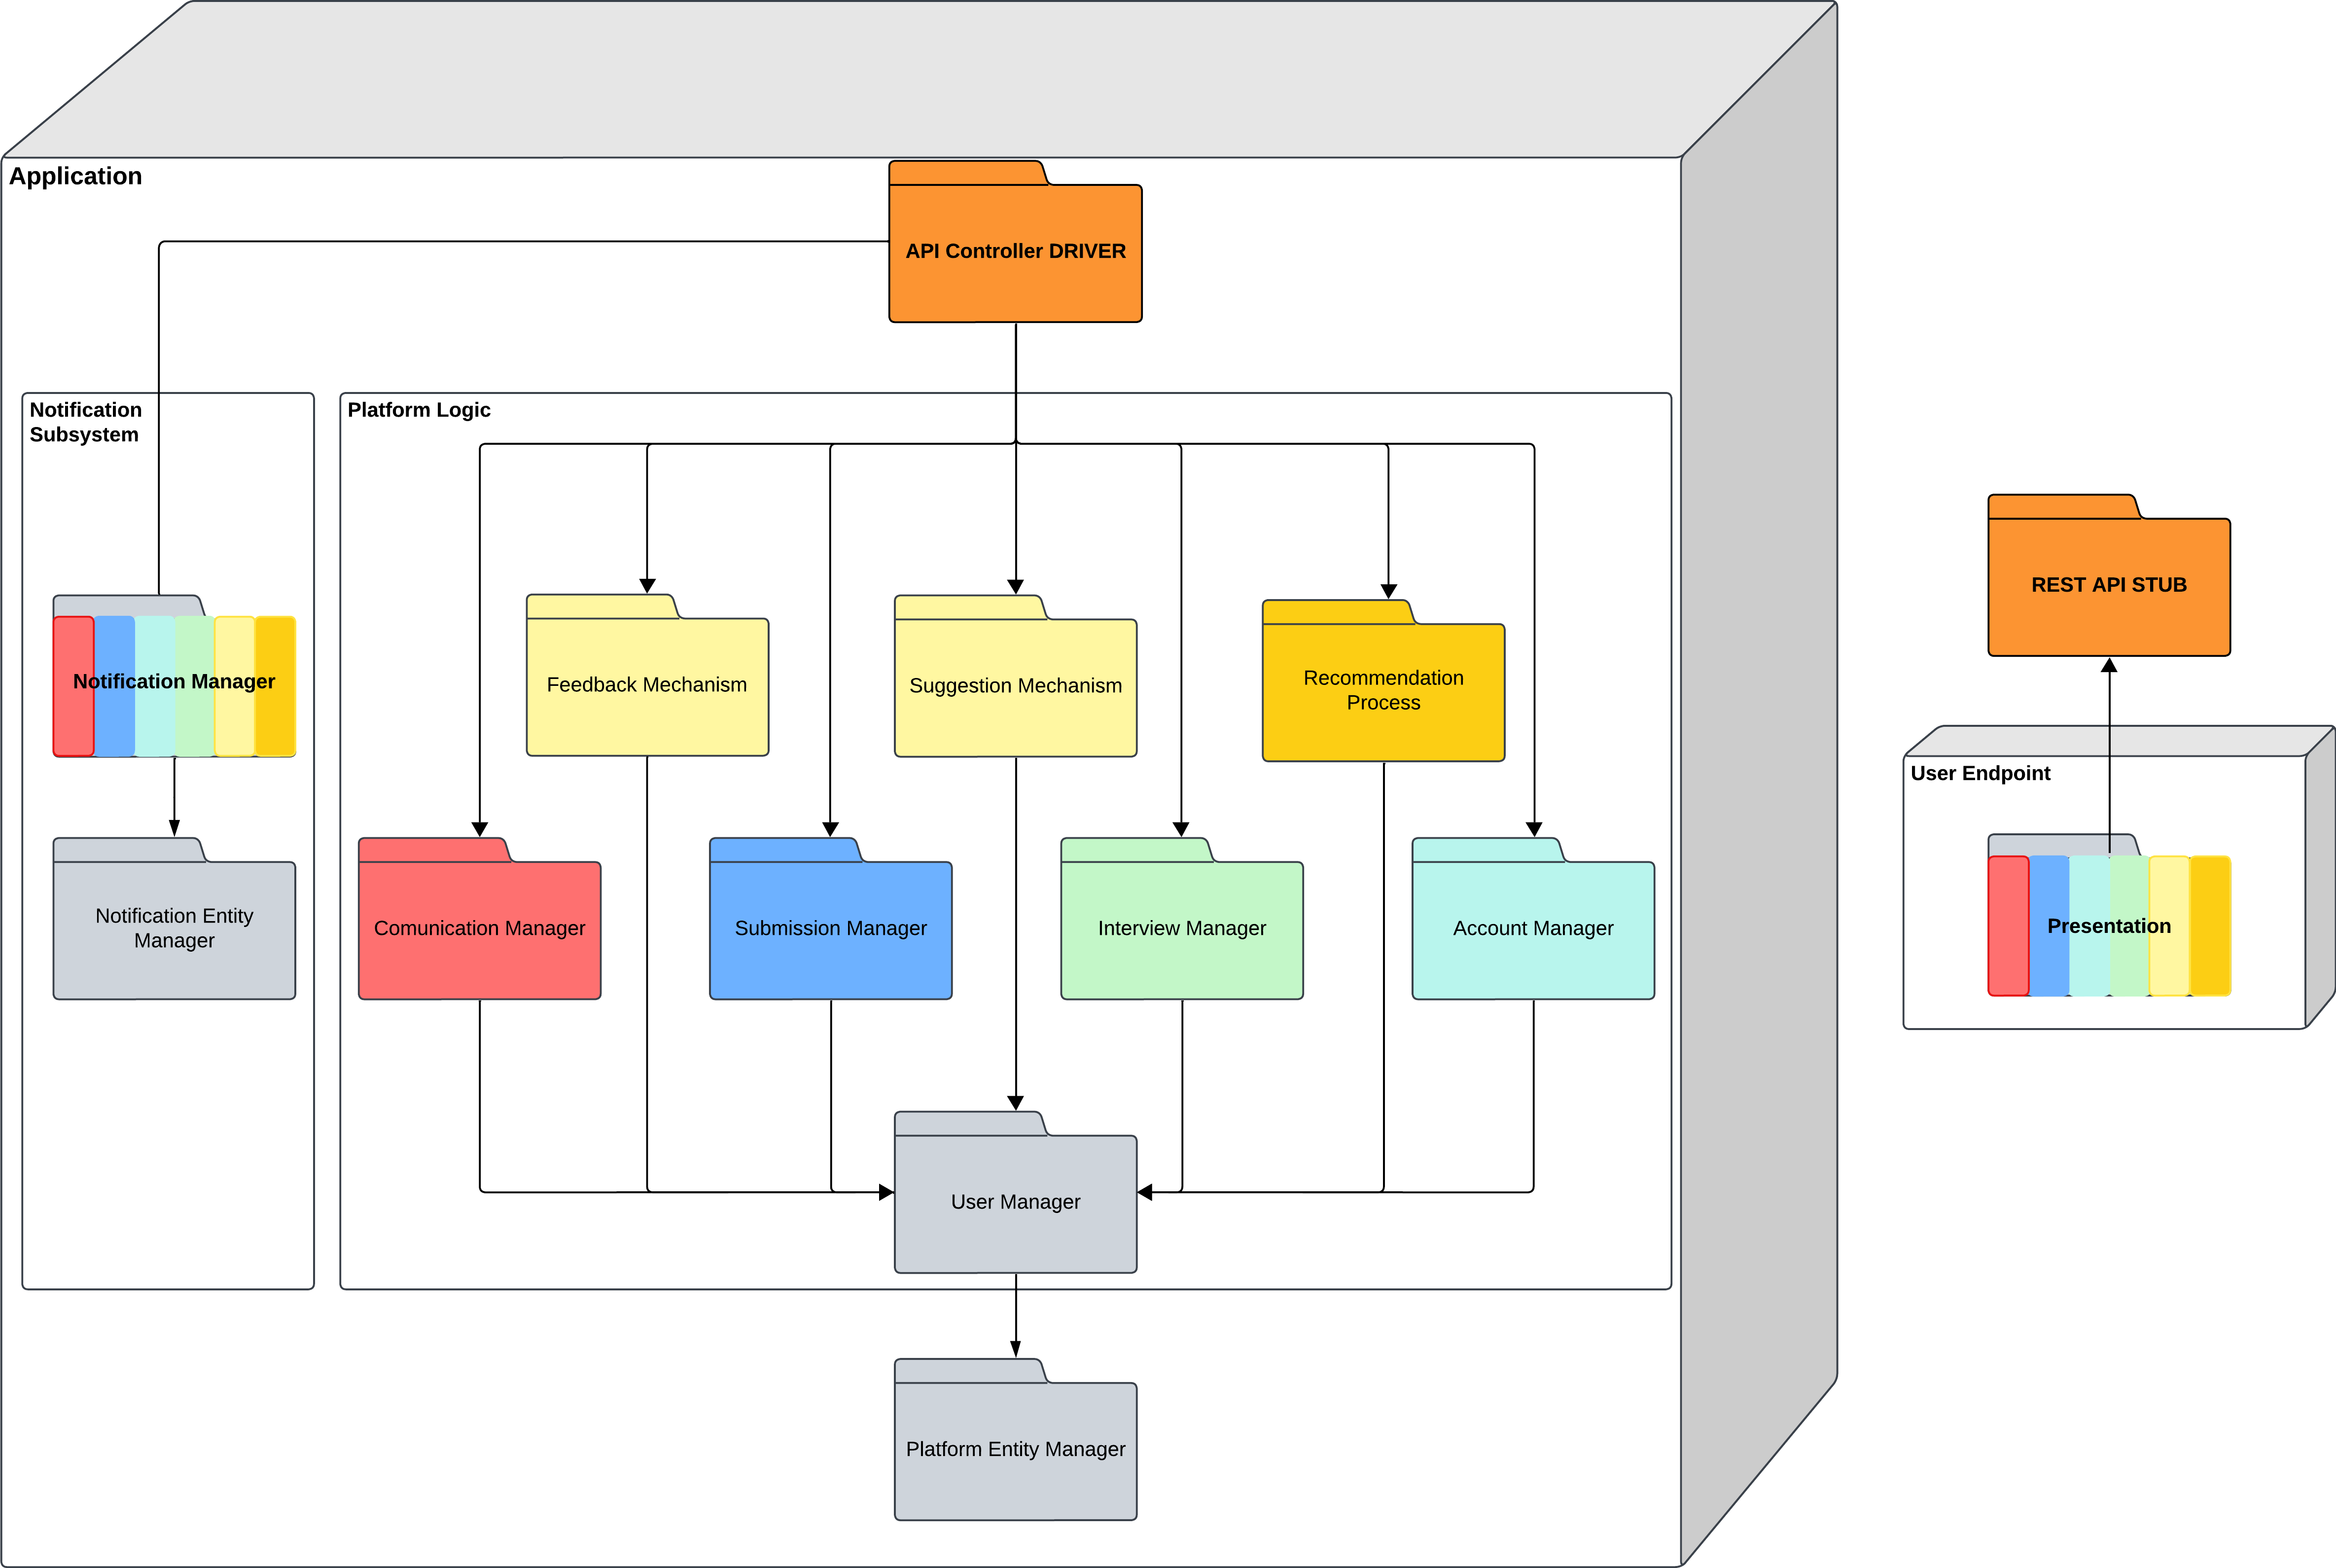
\includegraphics[width=\linewidth]{Latex/Images/DD/Testing/TestingPlanStep2.png}
    \caption{Platform Logic Components and User Interface testing}
    \label{fig:test-step2}
    \end{figure}
    
    \clearpage
    \subsubsection{Stage 3: API Controller and Front-End Integration}
    In the third stage, we will develop and integrate the API Controller with the Platform Logic components, the Notification Manager, and the User Interface that should have been completed in the previous stages. This will allow us to test the API Controller and the Platform Logic components together, ensuring that they interact correctly and that the API Controller can handle requests from the front-end and route them to the appropriate components.\\
    We will also develop the Authenticator Adapter to handle user authentication and token generation. For testing purpose we will create a Proxy DRIVER to simulate the API Controller and Authenticator Adapter calls and the front-end when it receives different responses.\\ 
    \begin{figure}[H]
    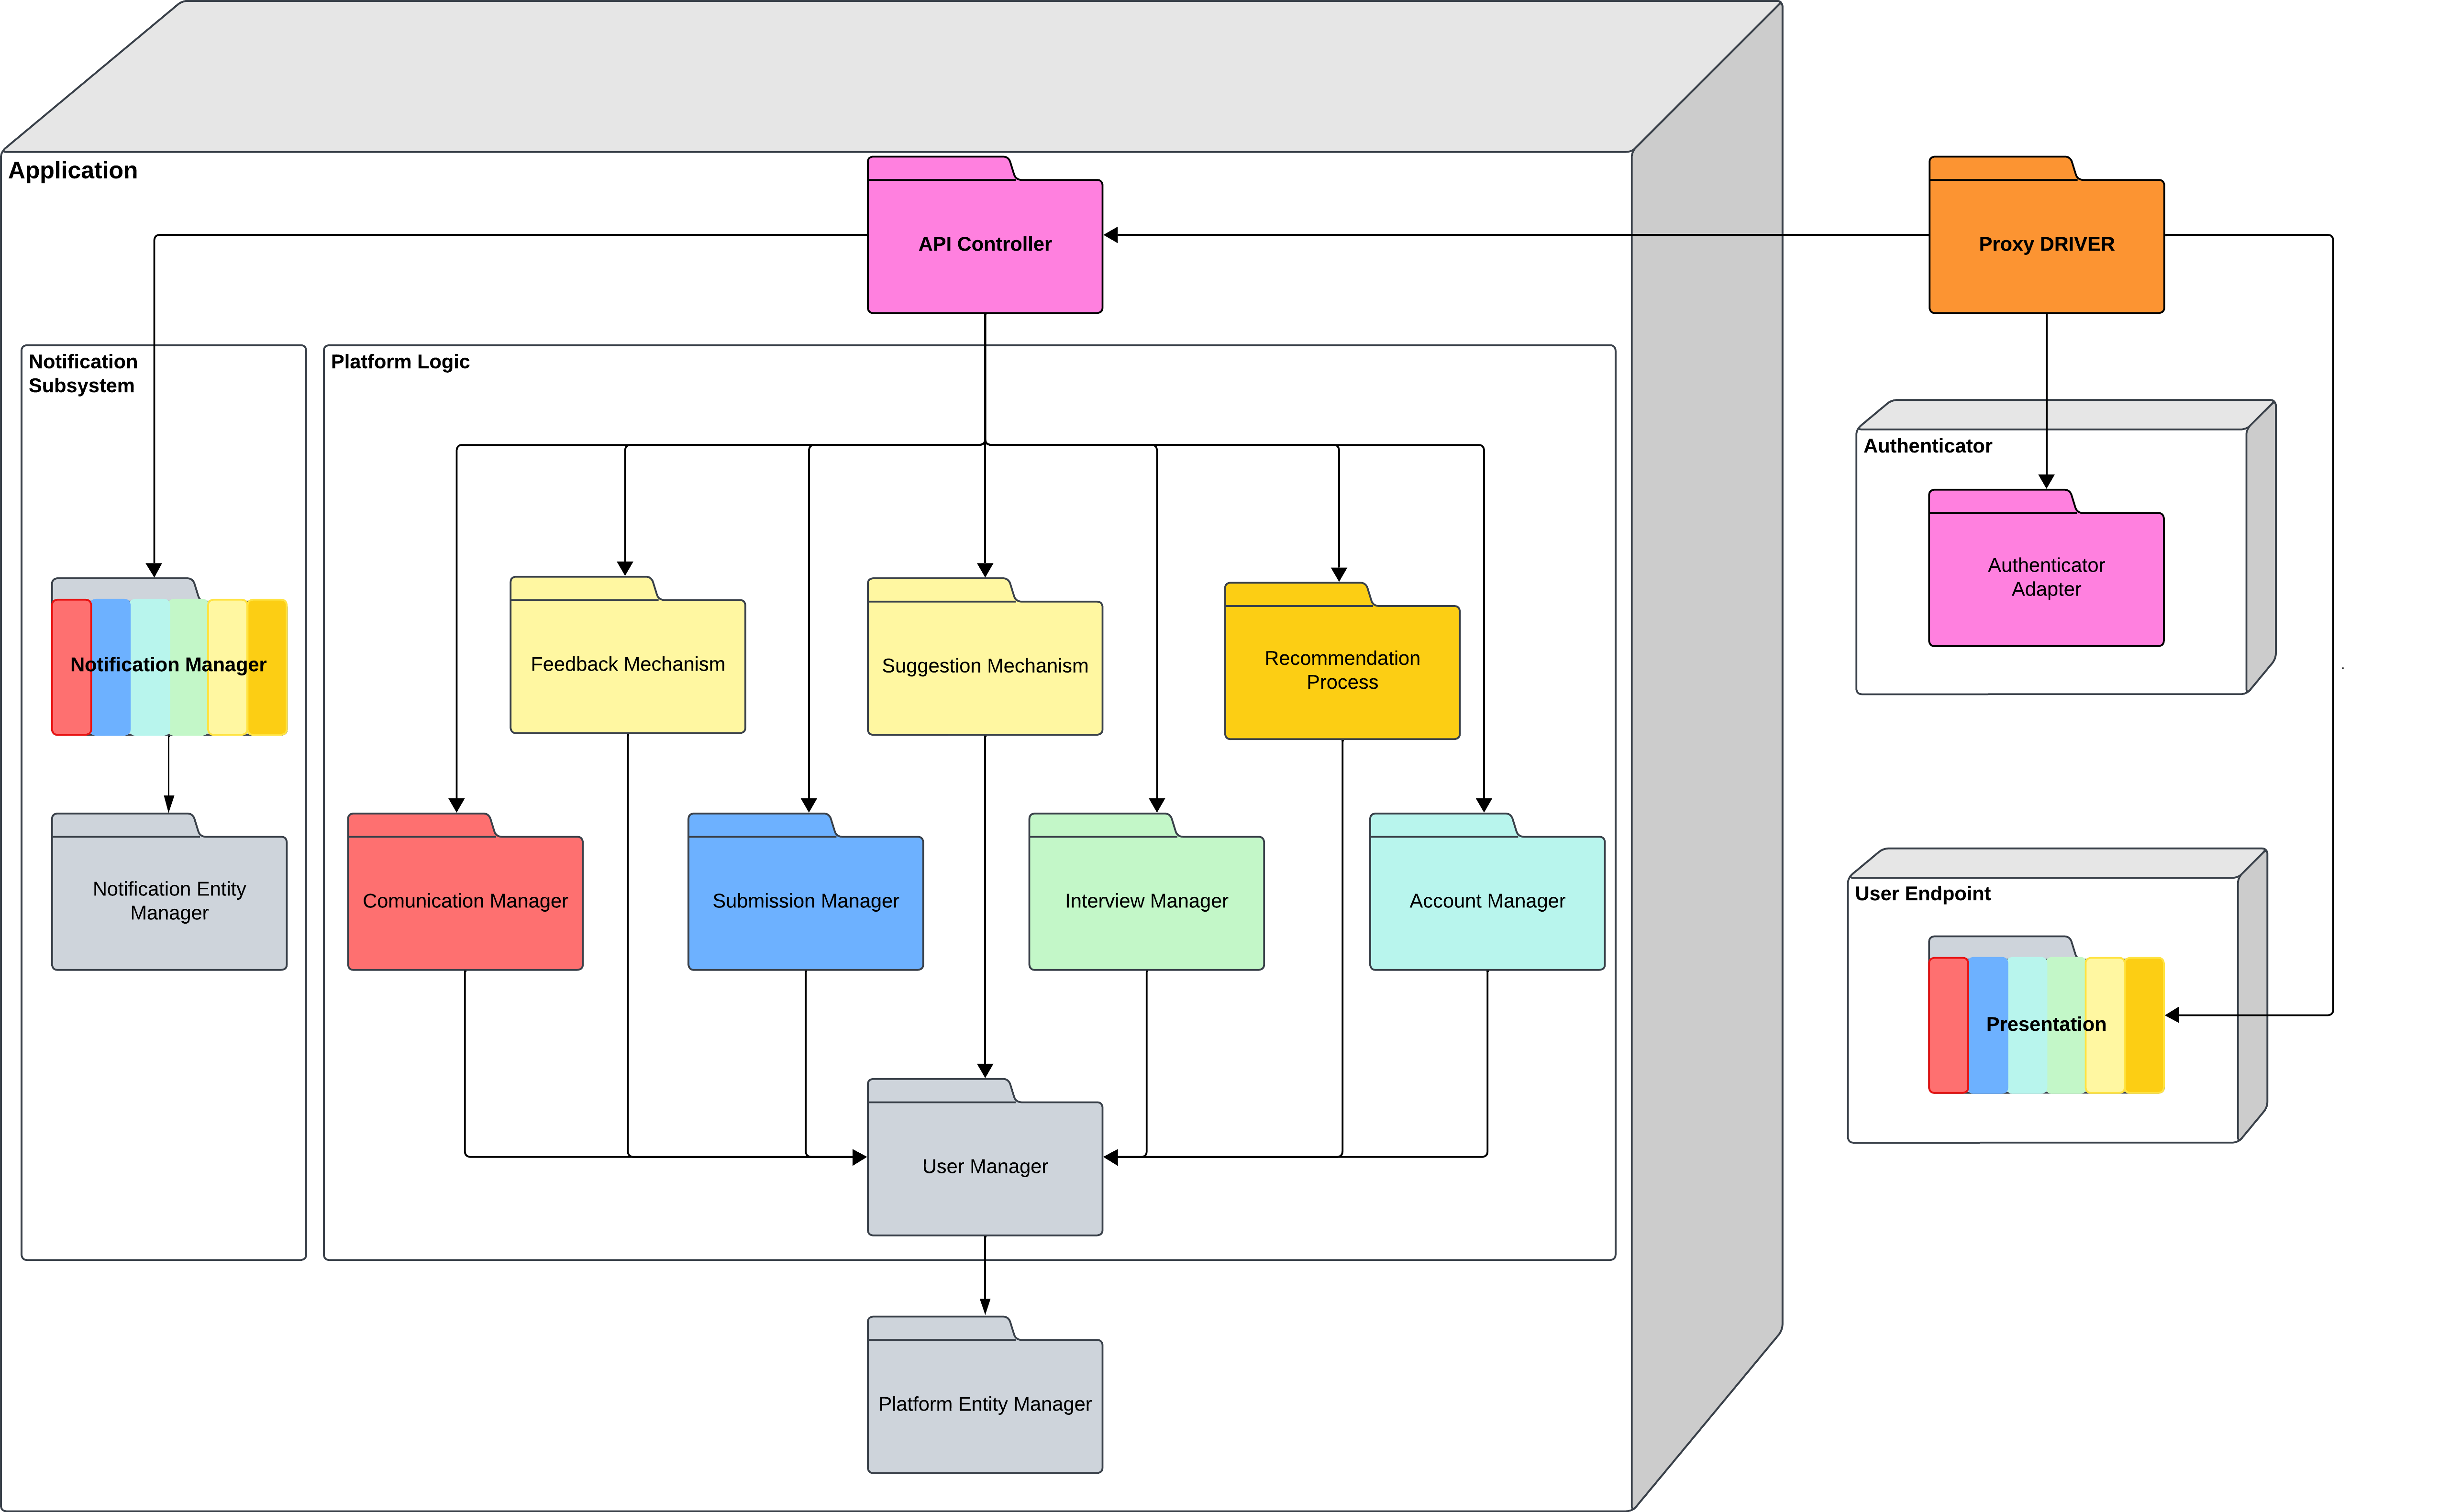
\includegraphics[width=\linewidth]{Latex/Images/DD/Testing/TestingPlanStep3.png}
    \caption{API Controller and Front-End Integration testing}
    \label{fig:test-step3}
    \end{figure}
    
    \clearpage
    \subsubsection{Stage 4: Full Integration and Testing}
    In the final stage, we will integrate all components of the platform thanks to the development of the Proxy and the Authenticator Adapter. This allows us to test the platform as a whole, ensuring that all components work together as expected. We will also conduct end-to-end testing to verify that the platform meets all requirements and functions correctly.
    \begin{figure}[H]
    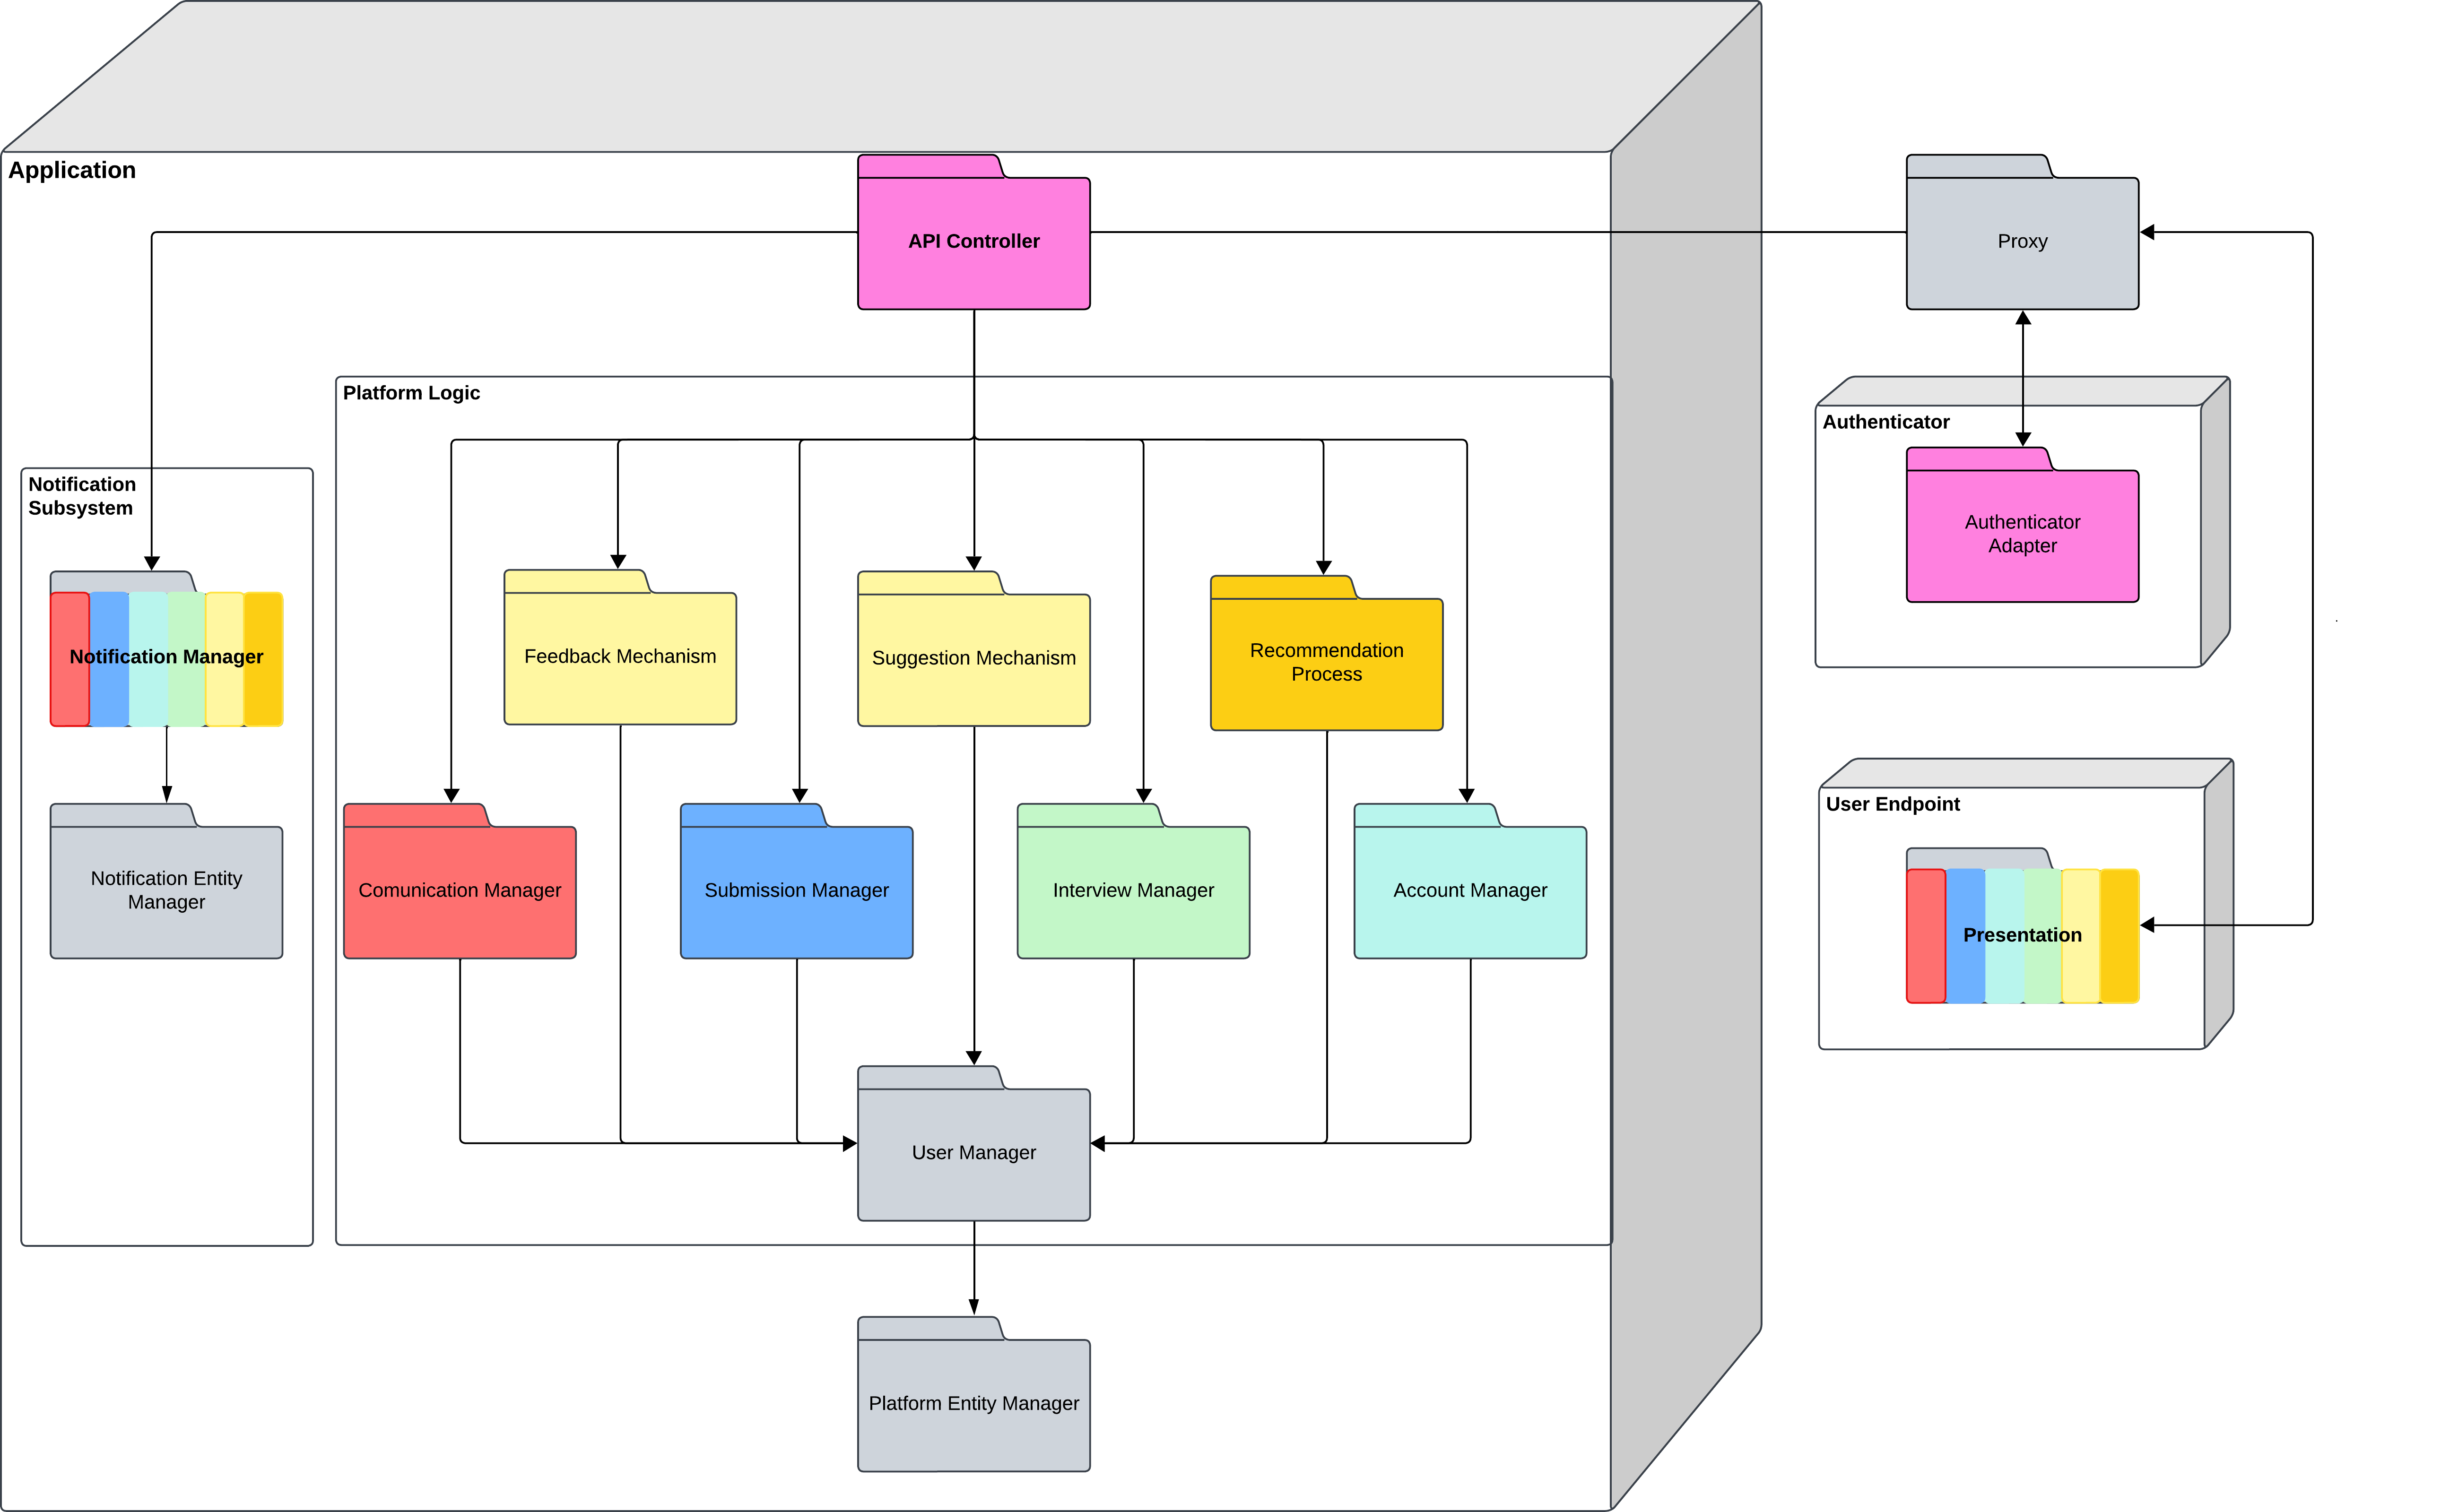
\includegraphics[width=\linewidth]{Latex/Images/DD/Testing/TestingPlanStep4.png}
    \caption{Full Integration and Testing}
    \label{fig:test-step4}
    \end{figure}
    \subsection{Technologies Used}
    In this last paragraph, we will describe the technologies used for the implementation, integration, and testing of the S\&C platform, discussing the reasons behind their choice and how they will be used in the development process.\\
    \subsubsection{Implementation Technologies}
    \begin{itemize}
        \item \textbf{Front-End}: The front-end of the platform will be developed using React, a popular JavaScript library for building user interfaces. React was chosen for its ease of use, flexibility, and performance, and wide support and documentation given the large community of developers that use it. The front-end will be styled using the MUI library to ensure a consistent and modern design across all pages and animated using the Framer Motion library.
        \item \textbf{Back-End}: The back-end of the platform will be developed using Java and Spring Boot, a popular framework for building Java-based web applications. Spring Boot was chosen robustness, and scalability, and the familiarity of the team with the Java language.
        \item \textbf{Database}: The platform's database will be established with MariaDB, a widely-used and open-source relational database management system. To engage with the database, we will utilize the Java Persistence API (JPA) alongside Hibernate, a object-relational mapping (ORM) framework for Java applications, which enables us to handle the data without manually crafting SQL queries.
        \item \textbf{Authentication}: Firebase Authentication, a reliable and popular service from Google, will be utilized to implement the authentication system for the platform. Firebase Auth was selected due to its easy of integration, scalability, and the range of authentication options it offers, such as email/password and logins via popular social networks like Facebook or Google.\\
        Moreover, Firebase Auth offers inherent security functionalities, including token-based authentication and secure user management, which correspond with our platform's requirement to manage sensitive information securely and efficiently
        \item \textbf{Notifications}: The platform’s notification system will be built with Firebase Cloud Messaging (FCM), a cross-platform messaging service that enables us to deliver push notifications to users on Android, iOS, and the web. FCM was selected for its dependability, scalability, and seamless integration with Firebase Auth, enabling us to send notifications securely and efficiently to platform users.
    \end{itemize}
    \subsubsection{Integration and Testing Technologies}
    \begin{itemize}
        \item \textbf{Unit Testing}: The platform's components of the back end will be tested using JUnit, a popular unit testing framework for Java applications.\\
        Moreover, JUnit was chosen for its simplicity, ease of use, compatibility with the Spring Boot framework and the team's familiarity with the tool.
        \item \textbf{Back-end Mock}: Mockito, a widely-used mocking framework for Java applications, will be used to create stub and mock objects for testing purposes.\\
        Moreover, Mockito was selected for its flexibility, ease of use, and compatibility with JUnit, allowing us both to simulate the behavior of external dependencies and to verify the interactions between components.
        \item \textbf{Front-end Testing}: The front-end of the platform will be tested using React Testing Library, a popular testing utility for React applications.\\
        Moreover, React Testing Library was chosen for the same reasons as React, and it allows us to write tests that closely resemble how users interact with the application, ensuring that the UI functions as expected.
        \item \textbf{Front-end Mock}: MSW (Mock Service Worker) will be used to mock the API calls made by the front-end during testing.\\
        Moreover, MSW was chosen for its ease of use, flexibility, and compatibility with React Testing Library, enabling us to simulate the behavior of the back-end components and test the front-end in isolation. 
    \end{itemize}